\documentclass{article}

\PassOptionsToPackage{numbers,compress}{natbib}
\usepackage{neurips_2024}

\usepackage[utf8]{inputenc}
\usepackage[T1]{fontenc}
\usepackage{hyperref}
\usepackage{url}
\usepackage{xurl}
\usepackage{graphicx}
\usepackage{booktabs}
\usepackage{tabularx}
\usepackage{array}
\usepackage{amsmath}
\usepackage{amssymb}
\usepackage{amsfonts}
\usepackage{nicefrac}
\usepackage{microtype}
\usepackage{xcolor}
\usepackage{float}
\usepackage{listings}
\usepackage{enumitem}
\usepackage{subcaption}
\usepackage{multirow}
\usepackage{tikz}

\graphicspath{{./}{../figures/}}

\lstset{
  basicstyle=\scriptsize\ttfamily,
  breaklines=true,
  frame=single,
  columns=fullflexible,
  backgroundcolor=\color{gray!5},
  showstringspaces=false
}

\title{Traffic Adaptive Network Guidance \& Optimization (TANGO)\\
\vspace{0.3em}
\small Team: Get Set TanGO \quad Workshop: \href{https://ieee-itsc.org/2026/}{IEEE ITSC 2026}}

\author{%
  Aryan Shrivastava \And
  Kotaro Murakami \And
  Yash Nishit Kapadia
}

\begin{document}

\maketitle

\begin{abstract}
This project set out to build a two-model traffic optimization system for a corridor of 12 signalized intersections in Toronto: a real-time controller (ASCE) and a scenario-planning surrogate (PIRA). Only ASCE was completed and evaluated; PIRA's pipeline runs end-to-end on synthetic data but did not converge on real ASCE rollouts within the project timeline and is not evaluated in this report. ASCE is an action-gate residual MAPPO controller that consistently outperforms Max-Pressure across four TMC-calibrated scenarios. Across 5 matched random seeds, paired-test reductions in person-time-loss relative to Max-Pressure are: AM Peak $-10.1\%$ ($p\!=\!0.003$); PM Peak $-6.3\%$ ($p\!=\!0.048$); Demand Surge $-11.0\%$ ($p\!=\!0.013$); Midday Multimodal $-13.8\%$ ($p\!=\!0.007$). ASCE also has the lowest mean person-time-loss against SUMO's auto-generated Actuated Default and a naive Fixed-Time controller on every scenario, although it is statistically tied with Actuated Default on three of four (significant gain only on AM Peak). Vehicle-delay fairness (Jain index) improves by ${\sim}30\%$ relative to Max-Pressure but remains below the proposal's aspirational 0.8 target. The project code and trained models are publicly available.\footnote{\url{https://github.com/yashnkapadia/ece324-TANGO}}
\end{abstract}

\section{Introduction}

Urban traffic congestion costs Toronto an estimated \$6 billion annually in lost productivity~\cite{cbc_gridlock}. This project was intended to be a two-model traffic optimization system for a corridor of 12 signalized intersections in Toronto, specifically aiming to reduce total delay (first layer, Adaptive Signal Control Engine or ``ASCE'') and help predict traffic change due to a change in the infrastructure (second layer, or Planning Infrastructure Response Analyzer ``PIRA'').

ASCE met its primary success criterion---however, building the PIRA layer, which depended on the completion of the ASCE layer, proved to be ambitious within the given timeframe. This report focuses on the design and results of ASCE, with PIRA's incomplete state documented in Section~\ref{sec:pira} and the Statement of Scope Changes.

There are two baseline signal cycling systems which ASCE aimed to beat: Fixed-Time and Max-Pressure. Fixed-Time is simply letting intersections run blindly on a predefined timer. This is the most basic (and cheapest) system that should be easy to beat with any kind of adaptive signalling. Max-Pressure~\cite{max_pressure_optimal} is a decentralized (i.e.\ each intersection has no access to global traffic data) heuristic-based algorithm that prioritizes relieving the road with higher traffic. While this model performs well under regular traffic conditions it was trained on, it fails to adapt under irregular conditions (e.g.\ lane closure, sports event, subway disruptions).

ASCE is a decentralized model, where each intersection acts as an independent agent. It takes the current state at each signal intersection, including but not limited to queue lengths, incoming arrivals, approach speeds, and time of day. It then chooses a safe next signal decision stating the next phase to be served and duration of the green signal. This model aims to reduce delay and prevent queues from backing into other streets, even under irregular conditions.

The second layer, PIRA (Planning Infrastructure Response Analyzer), was meant to model the effect of construction, lane closures, and new public transit lines on traffic. For each scenario, the model would estimate how demand and road capacity will change and then recommend practical updates to signal timing and phasing, using insight from the first layer. This model aims to solve the problem of turning proposed projects into data-driven signal changes that keep traffic moving smoothly during and after the disruption. Following the proposal, ASCE's success criterion is a $\geq$10\% reduction in person-time-loss relative to the Max-Pressure baseline (Section~\ref{sec:success}); PIRA was originally targeted to reach within the SUMO seed-noise floor (mean absolute percentage error $\leq$10\%) but was not evaluated as it is incomplete.

\section{Conditions of Success}
\label{sec:success}

For ASCE, the proposal criterion is that traffic engineering typically treats a 10\% delay reduction as practically meaningful:
\begin{equation}
  \mathrm{PTL}_{\mathrm{MAPPO}} \leq 0.90 \times \mathrm{PTL}_{\mathrm{Max\text{-}Pressure}},
  \label{eq:success}
\end{equation}
where PTL denotes person-time-loss: the sum of per-vehicle excess travel time over free-flow conditions (SUMO \texttt{timeLoss}), weighted by estimated person occupancy (1.3 per car, 30 per transit vehicle). Evaluation uses 5 random seeds per scenario.

For PIRA, the target is a mean absolute percentage error of at most 10\% across seeds, with inference under 5~seconds per scenario. As PIRA training is incomplete, this criterion is not evaluated in this report.


% =============================================================================
% DATA SECTION — Yash's section
% =============================================================================
\section{Data Pipeline and Simulation}
\label{sec:data}

This project uses two layers of data. The first layer is the City of Toronto Traffic Volumes Multimodal Intersection Turning Movement Counts (TMC) dataset~\cite{udc_tmc}, which records motor vehicle, bicycle, and pedestrian volumes at intersections in 15-minute intervals. The raw TMC dataset contains approximately 1 million samples dating back to 1980. Each record includes the intersection location, date, time period, approach direction, turning movement, and vehicle count. The second layer is a large simulated training dataset built on top of a real OpenStreetMap road network using the SUMO microsimulation platform~\cite{sumo_home}, calibrated against the TMC volumes to produce 1.94 million reinforcement learning training samples.

\subsection{Study Area}

This project focuses on signalized intersections along Dundas Street West in Toronto, Ontario, Canada, from the intersection at University Avenue to the intersection at Bathurst Street. The signalized intersections selected on this corridor are shown in Figure~\ref{fig:study-area}.

\begin{figure}[t]
  \centering
  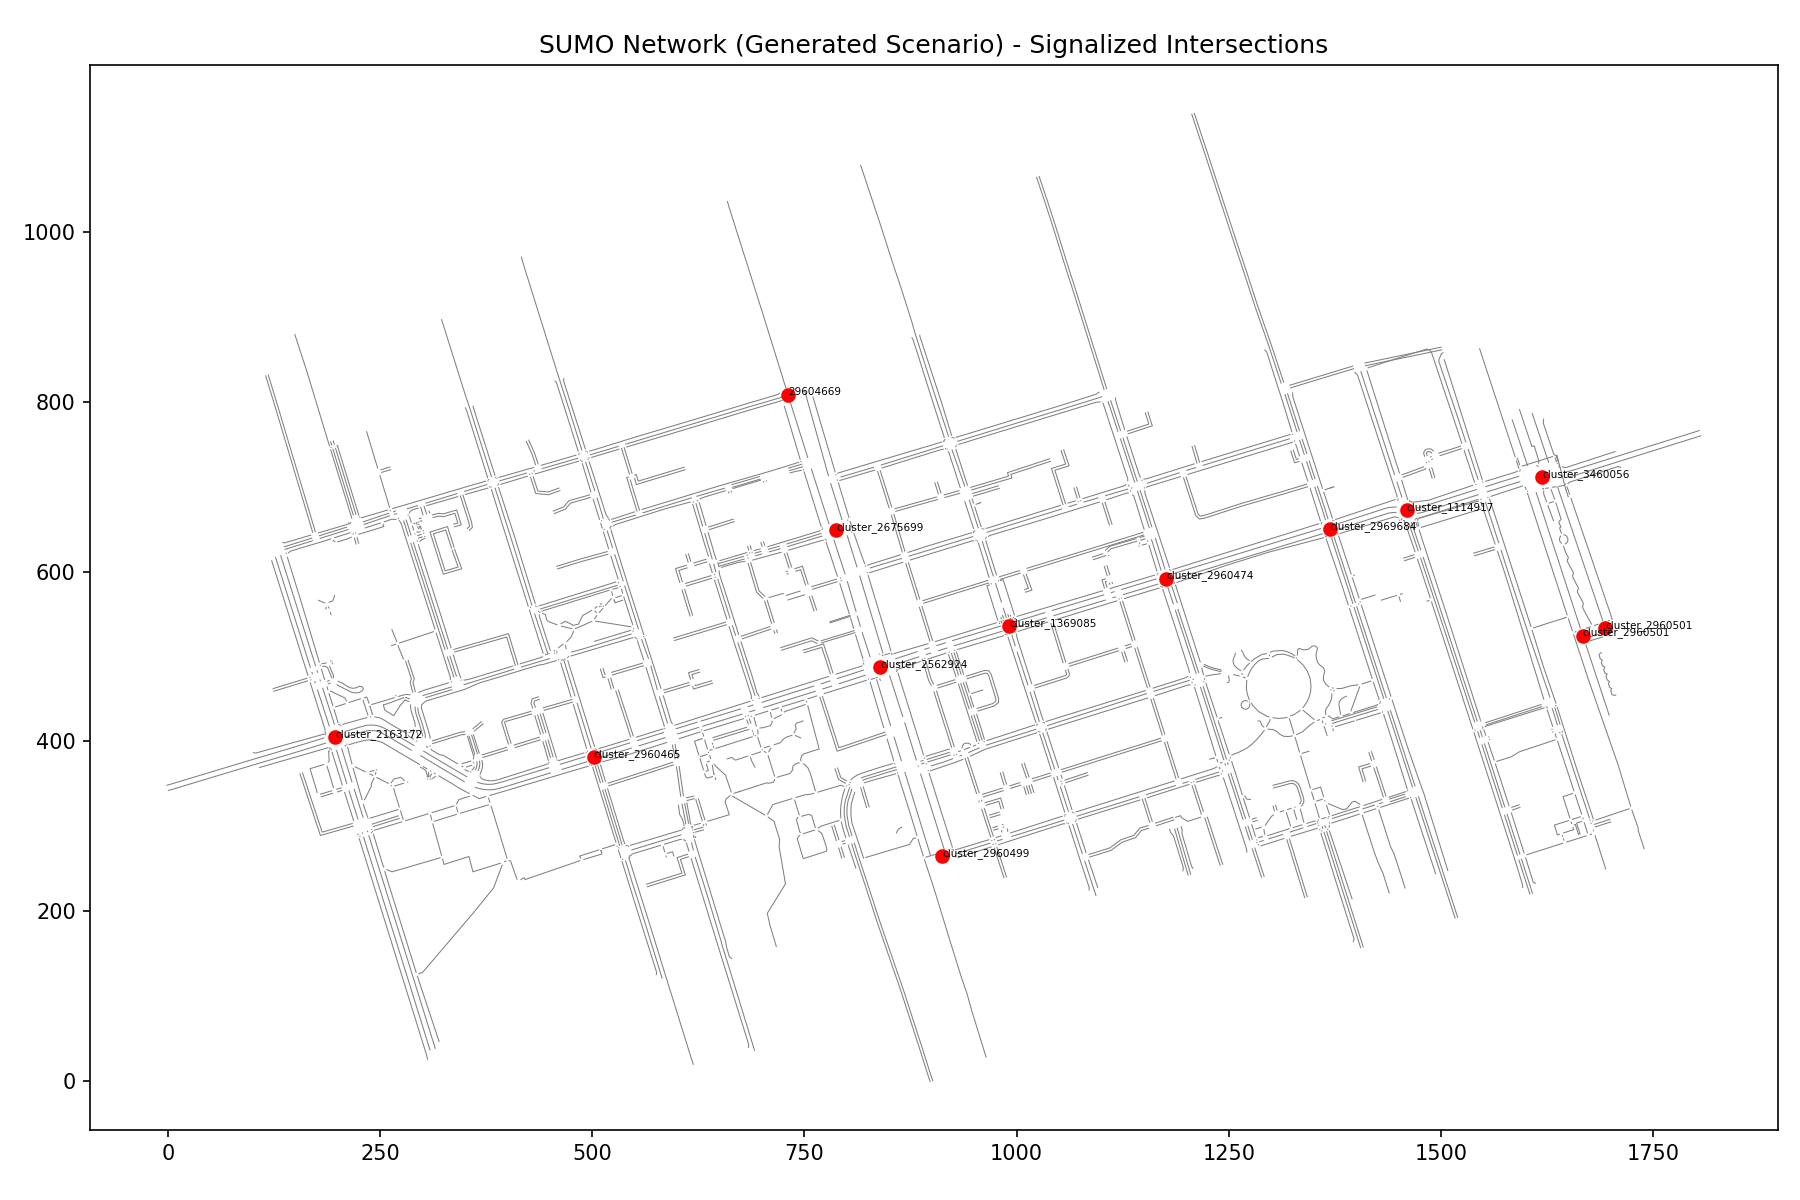
\includegraphics[width=0.85\columnwidth]{sumo_scenario_signalized_intersections.png}
  \caption{Generated SUMO scenario showing project area focus. The selected area is inspected using \texttt{sumolib} and annotated using \texttt{matplotlib} to highlight signalized intersections. The red markers indicate the locations of signalized intersections along the corridor.}
  \label{fig:study-area}
\end{figure}

This corridor was chosen because TMC data are available for it, it includes a streetcar route that is relevant for transit scenarios in the next phase of the project, and it is small enough (5 to 20 intersections) to iterate quickly while being large enough to capture signal coordination effects.

To support the simulated training dataset, the study area is first converted into a SUMO road network and then checked and corrected for signal control. The road network is created with the SUMO OSM Web Wizard~\cite{sumo_osm_wizard}, which pulls a bounding box from OpenStreetMap and produces a SUMO network file (\texttt{osm.net.xml}) that includes road segments (edges), intersections (junctions), lanes, connections, and traffic light programs. The bounding box covers roughly 200 meters north and south of Dundas Street between Bathurst and University. This network file is the first input to the MAPPO algorithm for training. After export, a mapping script links each known intersection to its corresponding SUMO junction by projecting geographic coordinates with \texttt{sumolib} and matching to the nearest junction ID. The result is an intersection map CSV that connects real intersection names to SUMO junction identifiers.

\subsection{Custom Demand Generation Interface (Demand Studio)}

After the network is prepared and mapped to real intersections, the next practical problem is turning observed counts into scenario files that can be run repeatedly for controller experiments. The custom Demand Studio interface was built for that step. It is a local Dash application that links a SUMO network file, visualizes the junction graph, maps TMC locations to nearby junctions, and generates new demand and scenario outputs from the parsed TMC dataset in one workflow. It was created to remove the manual loop of switching between separate SUMO tools, editing XML files by hand, and tracking experiment settings in separate notes. It also keeps the baseline files untouched by writing outputs to dedicated generated folders, which makes scenario iteration safer and easier to manage. For MAPPO work, this gives a single place to define the traffic scenario and the controller configuration that should be associated with that scenario.

Demand Studio combines demand creation, controller setup, and validation in one workflow from observed TMC counts to simulation-ready scenarios. In Demand settings, users select mapped TMC locations, set the maximum TMC-to-junction match distance, choose date policy and time window, define simulation begin and end, and include cars, trucks, buses, streetcars, and pedestrians with global and mode-specific scaling plus a bus-to-streetcar share. The app aggregates counts by approach and turning movement, converts them into SUMO \texttt{flow} and \texttt{personFlow} entries, and can enforce strict shortest-path checks to avoid invalid routes, which supports controlled construction of peak, off-peak, directional, and multimodal stress scenarios for MAPPO. In Signal and MAPPO settings, users choose MAPPO custom, baseline fixed time, or baseline max pressure, where fixed time generates a dedicated TLS additional file from EW and NS green, yellow, all-red, and offset settings with optional cluster-signal inclusion, while non fixed-time modes use the default TLS override file when available. Max-pressure parameters and MAPPO hyperparameters are saved in scenario metadata so demand design and controller assumptions stay coupled for reproducible experiments, even though training execution is outside this interface. Advanced settings improve transferability and quality control through tunable heading ranges for N, S, E, and W approach classification on irregular network geometry, editable vehicle dynamics for cars, trucks, buses, and streetcars without manual route XML edits, and an optional short SUMO validation run that catches route and configuration issues early.

Further details about the custom Demand Studio web interface, UI walkthrough, and usage are given in the project documentation.\footnote{\url{https://github.com/yashnkapadia/ece324-TANGO/blob/main/DATA.md}}

\subsection{Scenarios for ASCE Training}
\label{sec:scenarios}

We used four scenarios for ASCE training: \texttt{am\_peak}, \texttt{midday\_multimodal}, \texttt{pm\_peak}, and \texttt{demand\_surge}.

The \textbf{\texttt{am\_peak}} scenario is the reference case for ASCE training, meant to represent a relatively steady morning corridor where Max-Pressure is expected to perform well. Technically, it uses the latest parsed TMC data on the eight Dundas corridor intersections, with a morning window starting at minute 420 for 120 minutes, strict route checking enabled, and all five demand modes active with unit scaling. No artificial surge is added in Layer 2, while streetcars are still injected in both directions at a 360-second headway to keep regular transit pressure in the system. The run is configured with \texttt{simulation\_seconds} 900 and \texttt{simulation\_end} 1200, producing 174 vehicle flows and 8 pedestrian flows, with totals of 13{,}144 cars, 388 trucks, 168 buses, and 2{,}096 pedestrians.

The \textbf{\texttt{midday\_multimodal}} scenario is the high-conflict daytime case, designed to stress multimodal interactions rather than pure commuter car dominance. In plain terms, it captures the period where pedestrian and transit activity is strongest, including the documented Spadina pedestrian intensity in the rationale. In settings terms, it uses the latest TMC records with a midday window starting at minute 660 for 180 minutes, all five modes enabled, unit mode scales, no synthetic surge, and the same bidirectional 360-second streetcar injection pattern. It runs with \texttt{simulation\_seconds} 1200 and \texttt{simulation\_end} 1500 and yields 177 vehicle flows and 8 pedestrian flows, with high totals across modes, including 20{,}928 cars, 679 trucks, 179 buses, and 6{,}538 pedestrians.

The \textbf{\texttt{pm\_peak}} scenario represents the evening directional shift case, where demand pressure moves eastbound and pedestrian activity remains heavy. This scenario is configured from the latest TMC data using a PM window that starts at minute 960 and lasts 120 minutes, again with strict route checks, all five modes included, and no Layer 2 surge added. Transit pressure is kept comparable to the other base scenarios through 360-second eastbound and westbound streetcar injections. The configuration uses \texttt{simulation\_seconds} 900 and \texttt{simulation\_end} 1200 and generates 156 vehicle flows and 8 pedestrian flows, with totals of 18{,}810 cars, 239 trucks, 114 buses, and 5{,}347 pedestrians.

The \textbf{\texttt{demand\_surge}} scenario is the event dispersal case, built to test how ASCE handles a short, strong directional shock on top of PM conditions. It keeps the same PM base demand setup as \texttt{pm\_peak}, including latest TMC selection, \texttt{time\_window\_start} 960, \texttt{time\_window\_duration\_min} 120, full multimodal inclusion, and 360-second bidirectional streetcar injections, then adds a Layer 2 eastbound surge with multiplier 2.0 from second 300 to second 600. This isolates a temporary directional spike without changing the rest of the scenario structure. It runs longer, with \texttt{simulation\_seconds} 1200 and \texttt{simulation\_end} 1500, and produces 192 vehicle flows and 8 pedestrian flows, with totals of 19{,}630 cars, 252 trucks, 124 buses, and 5{,}347 pedestrians.

The ASCE section below describes how the four scenarios were used for MAPPO training.


% =============================================================================
% MODELING SECTION — Aryan's section
% =============================================================================
\section{Modeling}
\label{sec:modeling}

\subsection{Architecture: Action-Gate Residual MAPPO}

We adopt Multi-Agent Proximal Policy Optimization (MAPPO)~\cite{mappo} with parameter sharing, following the Centralized Training with Decentralized Execution (CTDE) paradigm as used in the CityLight framework~\cite{citylight}. Each of the 12 signalized intersections acts as an independent agent sharing a common policy network. A centralized critic, used only during training, receives the concatenated observations from all agents to estimate state value via Generalized Advantage Estimation~\cite{gae}.

For faster convergence and improved stability, the key architectural contribution is the \textbf{action-gate residual} design (Figure~\ref{fig:architecture}). At each time step, each agent receives a local observation concatenated with the Max-Pressure recommendation encoded as a one-hot vector. The shared actor network -- a 2-layer ReLU MLP with 128 hidden units -- produces two output heads:

\begin{itemize}[nosep]
  \item \textbf{Gate head} (2 outputs, softmax): a Bernoulli choice between \emph{follow Max-Pressure} and \emph{override with learned phase}.
  \item \textbf{Phase head} ($K$ outputs, softmax): a distribution over legal signal phases, masked to valid phases per intersection ($K \in \{2, \ldots, 6\}$).
\end{itemize}

The gate head is initialized with a bias of $[-2.0, +2.0]$, corresponding to an initial probability of approximately 98\% to follow Max-Pressure. This ensures the policy begins at Max-Pressure performance and focuses learning on situations where the heuristic is suboptimal. The action log-probability used for PPO updates is the joint log-probability of the gate decision and (if overriding) the phase selection, so both heads are trained end-to-end via a single PPO loss.

\begin{figure}[t]
  \centering
  \resizebox{\columnwidth}{!}{% ASCE Architecture Diagram — self-contained tikzpicture
% Usage: % ASCE Architecture Diagram — self-contained tikzpicture
% Usage: % ASCE Architecture Diagram — self-contained tikzpicture
% Usage: \input{asce_architecture.tex} inside a figure environment
% Requires: \usepackage{tikz} in the preamble
% Designed for NeurIPS two-column layout (\columnwidth ~ 3.25in)
\usetikzlibrary{arrows.meta, positioning, calc, backgrounds, fit}

% ---------------------------------------------------------------------------
% Colour palette
% ---------------------------------------------------------------------------
\definecolor{ascBlue}{HTML}{4393C3}
\definecolor{ascBlueFill}{HTML}{DAEAF6}
\definecolor{ascRed}{HTML}{C75B39}
\definecolor{ascRedFill}{HTML}{FBEAE4}
\definecolor{ascGreen}{HTML}{388E5E}
\definecolor{ascGreenFill}{HTML}{DFF0E7}
\definecolor{ascYellow}{HTML}{C8A028}
\definecolor{ascYellowFill}{HTML}{FFF3E0}
\definecolor{ascGrey}{HTML}{888888}
\definecolor{ascGreyFill}{HTML}{F0F0F0}

\begin{tikzpicture}[
    x=1cm, y=1cm,
    >={Stealth[length=2.5pt, width=2pt]},
    every node/.style={font=\sffamily},
    % --- node styles ---
    box/.style={
        draw, rounded corners=2pt, minimum height=0.6cm,
        inner sep=2.5pt, align=center,
        font=\sffamily\fontsize{7}{8.4}\selectfont,
    },
    inputbox/.style={box, fill=ascBlueFill, draw=ascBlue, text width=1.55cm},
    greybox/.style={box, fill=ascGreyFill, draw=ascGrey, minimum width=0.7cm},
    mlpbox/.style={box, fill=ascYellowFill, draw=ascYellow, line width=0.8pt,
                   text width=1.9cm, minimum height=0.8cm},
    gatebox/.style={box, fill=ascRedFill, draw=ascRed, text width=1.35cm},
    phasebox/.style={box, fill=ascGreenFill, draw=ascGreen, text width=1.35cm},
    actionbox/.style={box, draw=black!70, line width=0.7pt, text width=1.15cm},
    criticbox/.style={box, fill=ascBlueFill, draw=ascBlue, line width=0.8pt,
                      text width=2.0cm, minimum height=0.8cm},
    % --- annotation styles ---
    sub/.style={font=\sffamily\fontsize{5.5}{6.6}\selectfont,
                text=black!55, align=center, inner sep=0pt},
    arr/.style={->, semithick, color=black!60},
    trk/.style={font=\sffamily\bfseries\fontsize{6.5}{7.8}\selectfont,
                text=black!45},
]

% ===== ACTOR TRACK ==========================================================

\node[trk, anchor=west] at (0.15, 0.9)
    {ACTOR\enspace{\normalfont\fontsize{5.5}{6.6}\selectfont(per-agent, decentralized)}};

% -- Local Obs --
\node[inputbox] (lobs) at (1.0, 0) {Local Obs};
\node[sub, below=1.5pt of lobs.south, anchor=north, text width=2.0cm]
    {queue, density,\\phase, min-green};

% -- MP Action --
\node[greybox, text width=1.15cm] (mpact) at (1.0, -1.25) {MP Action};
\node[sub, below=1.5pt of mpact.south, anchor=north, text width=1.5cm]
    {one-hot\,|\,6\,dim};

% -- Concat --
\node[greybox, minimum width=0.5cm, minimum height=0.45cm,
      font=\sffamily\fontsize{7}{8.4}\selectfont] (cat) at (2.85, -0.55)
    {$\oplus$};

% -- Welford --
\node[greybox, text width=1.15cm] (welf) at (4.15, -0.55)
    {Welford $\mu/\sigma$};

% -- Shared MLP --
\node[mlpbox] (mlp) at (6.0, -0.55)
    {Shared MLP\\[-1pt]
     {\fontsize{5.5}{6.6}\selectfont 128\,$\to$\,ReLU}\\[-1pt]
     {\fontsize{5.5}{6.6}\selectfont 128\,$\to$\,ReLU}};
\node[sub, below=1.5pt of mlp.south, anchor=north]
    {$\times$12 agents};

% -- Gate Head --
\node[gatebox] (gate) at (8.15, 0.15) {Gate Head};
\node[sub, below=1.5pt of gate.south, anchor=north, text width=1.8cm]
    {follow / override\\init: 98\% follow};

% -- Phase Head --
\node[phasebox] (phase) at (8.15, -1.25) {Phase Head};
\node[sub, below=1.5pt of phase.south, anchor=north, text width=1.8cm]
    {6 phases (masked)\\softmax over valid};

% -- Action --
\node[actionbox] (act) at (9.85, -0.55) {Action};
\node[sub, below=1.5pt of act.south, anchor=north, text width=1.6cm]
    {{\color{ascRed}$g{=}0\!\to\!\mathrm{MP}$}\\
     {\color{ascGreen}$g{=}1\!\to\!\pi$}};

% -- Arrows: actor track --
\draw[arr] (lobs.east)  -- ++(0.2,0) |- (cat.west);
\draw[arr] (mpact.east) -- ++(0.2,0) |- (cat.west);
\draw[arr] (cat.east)   -- (welf.west);
\draw[arr] (welf.east)  -- (mlp.west);
\draw[arr] (mlp.east)   -- ++(0.2,0) |- (gate.west);
\draw[arr] (mlp.east)   -- ++(0.2,0) |- (phase.west);
\draw[arr] (gate.east)  -- ++(0.2,0) |- (act.west);
\draw[arr] (phase.east) -- ++(0.2,0) |- (act.west);


% ===== CTDE BOUNDARY ========================================================
\draw[dashed, black!35, line width=0.45pt] (0.0, -2.45) -- (10.7, -2.45);
\node[font=\sffamily\itshape\fontsize{5.5}{6.6}\selectfont, text=black!40,
      anchor=west] at (0.0, -2.65)
    {CTDE boundary --- critic used during training only};


% ===== CRITIC TRACK ==========================================================

\node[trk, anchor=west] at (0.15, -3.0)
    {CRITIC\enspace{\normalfont\fontsize{5.5}{6.6}\selectfont(centralized, training only)}};

% -- Global Obs --
\node[inputbox] (gobs) at (2.85, -3.8) {Global Obs};
\node[sub, below=1.5pt of gobs.south, anchor=north, text width=2.2cm]
    {all 12 agents\,|\,${\sim}$460\,d};

% -- Centralized Critic --
\node[criticbox] (crit) at (6.0, -3.8)
    {Centralized Critic\\[-1pt]
     {\fontsize{5.5}{6.6}\selectfont 128\,$\to$\,ReLU\,$\to$\,128}\\[-1pt]
     {\fontsize{5.5}{6.6}\selectfont $\to$\,ReLU\,$\to$\,1}};

% -- V(s) --
\node[actionbox, text width=0.7cm, minimum width=0.7cm] (vs) at (8.4, -3.8)
    {$V(s)$};
\node[sub, below=1.5pt of vs.south, anchor=north, text width=1.1cm]
    {scalar value};

% -- Arrows: critic track --
\draw[arr] (gobs.east) -- (crit.west);
\draw[arr] (crit.east) -- (vs.west);

\end{tikzpicture}
 inside a figure environment
% Requires: \usepackage{tikz} in the preamble
% Designed for NeurIPS two-column layout (\columnwidth ~ 3.25in)
\usetikzlibrary{arrows.meta, positioning, calc, backgrounds, fit}

% ---------------------------------------------------------------------------
% Colour palette
% ---------------------------------------------------------------------------
\definecolor{ascBlue}{HTML}{4393C3}
\definecolor{ascBlueFill}{HTML}{DAEAF6}
\definecolor{ascRed}{HTML}{C75B39}
\definecolor{ascRedFill}{HTML}{FBEAE4}
\definecolor{ascGreen}{HTML}{388E5E}
\definecolor{ascGreenFill}{HTML}{DFF0E7}
\definecolor{ascYellow}{HTML}{C8A028}
\definecolor{ascYellowFill}{HTML}{FFF3E0}
\definecolor{ascGrey}{HTML}{888888}
\definecolor{ascGreyFill}{HTML}{F0F0F0}

\begin{tikzpicture}[
    x=1cm, y=1cm,
    >={Stealth[length=2.5pt, width=2pt]},
    every node/.style={font=\sffamily},
    % --- node styles ---
    box/.style={
        draw, rounded corners=2pt, minimum height=0.6cm,
        inner sep=2.5pt, align=center,
        font=\sffamily\fontsize{7}{8.4}\selectfont,
    },
    inputbox/.style={box, fill=ascBlueFill, draw=ascBlue, text width=1.55cm},
    greybox/.style={box, fill=ascGreyFill, draw=ascGrey, minimum width=0.7cm},
    mlpbox/.style={box, fill=ascYellowFill, draw=ascYellow, line width=0.8pt,
                   text width=1.9cm, minimum height=0.8cm},
    gatebox/.style={box, fill=ascRedFill, draw=ascRed, text width=1.35cm},
    phasebox/.style={box, fill=ascGreenFill, draw=ascGreen, text width=1.35cm},
    actionbox/.style={box, draw=black!70, line width=0.7pt, text width=1.15cm},
    criticbox/.style={box, fill=ascBlueFill, draw=ascBlue, line width=0.8pt,
                      text width=2.0cm, minimum height=0.8cm},
    % --- annotation styles ---
    sub/.style={font=\sffamily\fontsize{5.5}{6.6}\selectfont,
                text=black!55, align=center, inner sep=0pt},
    arr/.style={->, semithick, color=black!60},
    trk/.style={font=\sffamily\bfseries\fontsize{6.5}{7.8}\selectfont,
                text=black!45},
]

% ===== ACTOR TRACK ==========================================================

\node[trk, anchor=west] at (0.15, 0.9)
    {ACTOR\enspace{\normalfont\fontsize{5.5}{6.6}\selectfont(per-agent, decentralized)}};

% -- Local Obs --
\node[inputbox] (lobs) at (1.0, 0) {Local Obs};
\node[sub, below=1.5pt of lobs.south, anchor=north, text width=2.0cm]
    {queue, density,\\phase, min-green};

% -- MP Action --
\node[greybox, text width=1.15cm] (mpact) at (1.0, -1.25) {MP Action};
\node[sub, below=1.5pt of mpact.south, anchor=north, text width=1.5cm]
    {one-hot\,|\,6\,dim};

% -- Concat --
\node[greybox, minimum width=0.5cm, minimum height=0.45cm,
      font=\sffamily\fontsize{7}{8.4}\selectfont] (cat) at (2.85, -0.55)
    {$\oplus$};

% -- Welford --
\node[greybox, text width=1.15cm] (welf) at (4.15, -0.55)
    {Welford $\mu/\sigma$};

% -- Shared MLP --
\node[mlpbox] (mlp) at (6.0, -0.55)
    {Shared MLP\\[-1pt]
     {\fontsize{5.5}{6.6}\selectfont 128\,$\to$\,ReLU}\\[-1pt]
     {\fontsize{5.5}{6.6}\selectfont 128\,$\to$\,ReLU}};
\node[sub, below=1.5pt of mlp.south, anchor=north]
    {$\times$12 agents};

% -- Gate Head --
\node[gatebox] (gate) at (8.15, 0.15) {Gate Head};
\node[sub, below=1.5pt of gate.south, anchor=north, text width=1.8cm]
    {follow / override\\init: 98\% follow};

% -- Phase Head --
\node[phasebox] (phase) at (8.15, -1.25) {Phase Head};
\node[sub, below=1.5pt of phase.south, anchor=north, text width=1.8cm]
    {6 phases (masked)\\softmax over valid};

% -- Action --
\node[actionbox] (act) at (9.85, -0.55) {Action};
\node[sub, below=1.5pt of act.south, anchor=north, text width=1.6cm]
    {{\color{ascRed}$g{=}0\!\to\!\mathrm{MP}$}\\
     {\color{ascGreen}$g{=}1\!\to\!\pi$}};

% -- Arrows: actor track --
\draw[arr] (lobs.east)  -- ++(0.2,0) |- (cat.west);
\draw[arr] (mpact.east) -- ++(0.2,0) |- (cat.west);
\draw[arr] (cat.east)   -- (welf.west);
\draw[arr] (welf.east)  -- (mlp.west);
\draw[arr] (mlp.east)   -- ++(0.2,0) |- (gate.west);
\draw[arr] (mlp.east)   -- ++(0.2,0) |- (phase.west);
\draw[arr] (gate.east)  -- ++(0.2,0) |- (act.west);
\draw[arr] (phase.east) -- ++(0.2,0) |- (act.west);


% ===== CTDE BOUNDARY ========================================================
\draw[dashed, black!35, line width=0.45pt] (0.0, -2.45) -- (10.7, -2.45);
\node[font=\sffamily\itshape\fontsize{5.5}{6.6}\selectfont, text=black!40,
      anchor=west] at (0.0, -2.65)
    {CTDE boundary --- critic used during training only};


% ===== CRITIC TRACK ==========================================================

\node[trk, anchor=west] at (0.15, -3.0)
    {CRITIC\enspace{\normalfont\fontsize{5.5}{6.6}\selectfont(centralized, training only)}};

% -- Global Obs --
\node[inputbox] (gobs) at (2.85, -3.8) {Global Obs};
\node[sub, below=1.5pt of gobs.south, anchor=north, text width=2.2cm]
    {all 12 agents\,|\,${\sim}$460\,d};

% -- Centralized Critic --
\node[criticbox] (crit) at (6.0, -3.8)
    {Centralized Critic\\[-1pt]
     {\fontsize{5.5}{6.6}\selectfont 128\,$\to$\,ReLU\,$\to$\,128}\\[-1pt]
     {\fontsize{5.5}{6.6}\selectfont $\to$\,ReLU\,$\to$\,1}};

% -- V(s) --
\node[actionbox, text width=0.7cm, minimum width=0.7cm] (vs) at (8.4, -3.8)
    {$V(s)$};
\node[sub, below=1.5pt of vs.south, anchor=north, text width=1.1cm]
    {scalar value};

% -- Arrows: critic track --
\draw[arr] (gobs.east) -- (crit.west);
\draw[arr] (crit.east) -- (vs.west);

\end{tikzpicture}
 inside a figure environment
% Requires: \usepackage{tikz} in the preamble
% Designed for NeurIPS two-column layout (\columnwidth ~ 3.25in)
\usetikzlibrary{arrows.meta, positioning, calc, backgrounds, fit}

% ---------------------------------------------------------------------------
% Colour palette
% ---------------------------------------------------------------------------
\definecolor{ascBlue}{HTML}{4393C3}
\definecolor{ascBlueFill}{HTML}{DAEAF6}
\definecolor{ascRed}{HTML}{C75B39}
\definecolor{ascRedFill}{HTML}{FBEAE4}
\definecolor{ascGreen}{HTML}{388E5E}
\definecolor{ascGreenFill}{HTML}{DFF0E7}
\definecolor{ascYellow}{HTML}{C8A028}
\definecolor{ascYellowFill}{HTML}{FFF3E0}
\definecolor{ascGrey}{HTML}{888888}
\definecolor{ascGreyFill}{HTML}{F0F0F0}

\begin{tikzpicture}[
    x=1cm, y=1cm,
    >={Stealth[length=2.5pt, width=2pt]},
    every node/.style={font=\sffamily},
    % --- node styles ---
    box/.style={
        draw, rounded corners=2pt, minimum height=0.6cm,
        inner sep=2.5pt, align=center,
        font=\sffamily\fontsize{7}{8.4}\selectfont,
    },
    inputbox/.style={box, fill=ascBlueFill, draw=ascBlue, text width=1.55cm},
    greybox/.style={box, fill=ascGreyFill, draw=ascGrey, minimum width=0.7cm},
    mlpbox/.style={box, fill=ascYellowFill, draw=ascYellow, line width=0.8pt,
                   text width=1.9cm, minimum height=0.8cm},
    gatebox/.style={box, fill=ascRedFill, draw=ascRed, text width=1.35cm},
    phasebox/.style={box, fill=ascGreenFill, draw=ascGreen, text width=1.35cm},
    actionbox/.style={box, draw=black!70, line width=0.7pt, text width=1.15cm},
    criticbox/.style={box, fill=ascBlueFill, draw=ascBlue, line width=0.8pt,
                      text width=2.0cm, minimum height=0.8cm},
    % --- annotation styles ---
    sub/.style={font=\sffamily\fontsize{5.5}{6.6}\selectfont,
                text=black!55, align=center, inner sep=0pt},
    arr/.style={->, semithick, color=black!60},
    trk/.style={font=\sffamily\bfseries\fontsize{6.5}{7.8}\selectfont,
                text=black!45},
]

% ===== ACTOR TRACK ==========================================================

\node[trk, anchor=west] at (0.15, 0.9)
    {ACTOR\enspace{\normalfont\fontsize{5.5}{6.6}\selectfont(per-agent, decentralized)}};

% -- Local Obs --
\node[inputbox] (lobs) at (1.0, 0) {Local Obs};
\node[sub, below=1.5pt of lobs.south, anchor=north, text width=2.0cm]
    {queue, density,\\phase, min-green};

% -- MP Action --
\node[greybox, text width=1.15cm] (mpact) at (1.0, -1.25) {MP Action};
\node[sub, below=1.5pt of mpact.south, anchor=north, text width=1.5cm]
    {one-hot\,|\,6\,dim};

% -- Concat --
\node[greybox, minimum width=0.5cm, minimum height=0.45cm,
      font=\sffamily\fontsize{7}{8.4}\selectfont] (cat) at (2.85, -0.55)
    {$\oplus$};

% -- Welford --
\node[greybox, text width=1.15cm] (welf) at (4.15, -0.55)
    {Welford $\mu/\sigma$};

% -- Shared MLP --
\node[mlpbox] (mlp) at (6.0, -0.55)
    {Shared MLP\\[-1pt]
     {\fontsize{5.5}{6.6}\selectfont 128\,$\to$\,ReLU}\\[-1pt]
     {\fontsize{5.5}{6.6}\selectfont 128\,$\to$\,ReLU}};
\node[sub, below=1.5pt of mlp.south, anchor=north]
    {$\times$12 agents};

% -- Gate Head --
\node[gatebox] (gate) at (8.15, 0.15) {Gate Head};
\node[sub, below=1.5pt of gate.south, anchor=north, text width=1.8cm]
    {follow / override\\init: 98\% follow};

% -- Phase Head --
\node[phasebox] (phase) at (8.15, -1.25) {Phase Head};
\node[sub, below=1.5pt of phase.south, anchor=north, text width=1.8cm]
    {6 phases (masked)\\softmax over valid};

% -- Action --
\node[actionbox] (act) at (9.85, -0.55) {Action};
\node[sub, below=1.5pt of act.south, anchor=north, text width=1.6cm]
    {{\color{ascRed}$g{=}0\!\to\!\mathrm{MP}$}\\
     {\color{ascGreen}$g{=}1\!\to\!\pi$}};

% -- Arrows: actor track --
\draw[arr] (lobs.east)  -- ++(0.2,0) |- (cat.west);
\draw[arr] (mpact.east) -- ++(0.2,0) |- (cat.west);
\draw[arr] (cat.east)   -- (welf.west);
\draw[arr] (welf.east)  -- (mlp.west);
\draw[arr] (mlp.east)   -- ++(0.2,0) |- (gate.west);
\draw[arr] (mlp.east)   -- ++(0.2,0) |- (phase.west);
\draw[arr] (gate.east)  -- ++(0.2,0) |- (act.west);
\draw[arr] (phase.east) -- ++(0.2,0) |- (act.west);


% ===== CTDE BOUNDARY ========================================================
\draw[dashed, black!35, line width=0.45pt] (0.0, -2.45) -- (10.7, -2.45);
\node[font=\sffamily\itshape\fontsize{5.5}{6.6}\selectfont, text=black!40,
      anchor=west] at (0.0, -2.65)
    {CTDE boundary --- critic used during training only};


% ===== CRITIC TRACK ==========================================================

\node[trk, anchor=west] at (0.15, -3.0)
    {CRITIC\enspace{\normalfont\fontsize{5.5}{6.6}\selectfont(centralized, training only)}};

% -- Global Obs --
\node[inputbox] (gobs) at (2.85, -3.8) {Global Obs};
\node[sub, below=1.5pt of gobs.south, anchor=north, text width=2.2cm]
    {all 12 agents\,|\,${\sim}$460\,d};

% -- Centralized Critic --
\node[criticbox] (crit) at (6.0, -3.8)
    {Centralized Critic\\[-1pt]
     {\fontsize{5.5}{6.6}\selectfont 128\,$\to$\,ReLU\,$\to$\,128}\\[-1pt]
     {\fontsize{5.5}{6.6}\selectfont $\to$\,ReLU\,$\to$\,1}};

% -- V(s) --
\node[actionbox, text width=0.7cm, minimum width=0.7cm] (vs) at (8.4, -3.8)
    {$V(s)$};
\node[sub, below=1.5pt of vs.south, anchor=north, text width=1.1cm]
    {scalar value};

% -- Arrows: critic track --
\draw[arr] (gobs.east) -- (crit.west);
\draw[arr] (crit.east) -- (vs.west);

\end{tikzpicture}
}
  \caption{Action-gate residual MAPPO architecture. The actor (top) processes local observations augmented with the Max-Pressure recommendation and produces a gate decision (follow or override) and a phase selection. The centralized critic (bottom) is used during training only. All 12 intersection agents share the same actor and critic parameters.}
  \label{fig:architecture}
\end{figure}

\paragraph{Observations.} Each agent observes local traffic state: current phase, per-lane density and queue fractions, and the Max-Pressure recommended phase as a one-hot vector. Feature dimensions vary by intersection topology (15 to 49 after padding); full details appear in Appendix~\ref{app:obs_features}. Features are normalized online using Welford's running mean and variance~\cite{welford}. The centralized critic receives all 12 agents' observations concatenated (${\sim}460$ dimensions) and is discarded at deployment.


\subsection{Reward Design}
\label{sec:reward}

The reward function underwent three iterations (detailed in Appendix~\ref{app:reward_iterations}). The interim report's multi-objective reward---combining delay, throughput, and global fairness---left MAPPO 25\% behind Max-Pressure because the throughput term dominated the delay gradient. An intermediate attempt to normalize person-weighted throughput into the reward amplified the problem further.

The final reward, \texttt{person\_objective}, removes throughput entirely and instead makes the delay signal richer:
\begin{equation}
  r_i = -\log\!\left(1 + \frac{\sum_v w_v \cdot t_v}{\sum_v w_v}\right) + 0.25 \cdot J\!\left(D_{\mathrm{NS}}^{(i)},\, D_{\mathrm{EW}}^{(i)}\right),
  \label{eq:reward_person}
\end{equation}
where the sum is over vehicles $v$ on edges approaching intersection $i$, $w_v$ is the person occupancy weight (1.3 for cars, 30.0 for transit), $t_v$ is the waiting time, $D_{\mathrm{NS}}^{(i)}$ and $D_{\mathrm{EW}}^{(i)}$ are person-weighted delays on the north--south and east--west approaches, and $J(\cdot)$ is the two-element Jain index. Dividing person-delay by person-throughput yields a per-person delay \emph{rate} that scales naturally with traffic volume. The local directional Jain term is directly actionable per agent, unlike the global throughput fairness used at interim. Person weighting aligns the reward with the evaluation KPI.


\subsection{Training Pipeline}
\label{sec:training}

Training proceeds in two phases, both using the \texttt{person\_objective} reward.

\paragraph{Phase 1: Warm-start (200 episodes, AM Peak only).}
The policy is trained from scratch on the AM Peak scenario to establish basic signal coordination before encountering harder scenarios. This phase uses a single SUMO worker and base learning rates (actor: $3 \times 10^{-4}$, critic: $1 \times 10^{-3}$). By episode 200, MAPPO achieves a person-time-loss ratio of approximately 0.90 relative to Max-Pressure on the AM Peak scenario.

\paragraph{Phase 2: Curriculum training (600 episodes, 4 scenarios).}
Starting from the warm-start checkpoint, the policy trains on all four scenarios from Section~\ref{sec:scenarios} in round-robin order, using 8 parallel SUMO workers via Python multiprocessing with \texttt{libsumo}. Learning rates are scaled by $1/\sqrt{8}$ to compensate for the larger effective batch size from parallel collection (square-root scaling rule of~\citet{hoffer_train_longer}), yielding actor $1.06 \times 10^{-4}$ and critic $3.54 \times 10^{-4}$. Episodes run for 900\,s (AM/PM Peak) or 1200\,s (Demand Surge, Midday Multimodal) at 5\,s decision intervals.

A best-model checkpoint is saved whenever inline evaluation (run every 48 episodes) achieves a new minimum worst-case MAPPO/MP ratio across all four scenarios. The best checkpoint occurs at curriculum episode 432 (total episode 632), after which training regresses due to conflicting gradient directions across scenarios---a known challenge in round-robin curriculum training. The final model (episode 600) performs measurably worse than the best checkpoint (Table~\ref{tab:results}), confirming that early stopping on worst-case evaluation is essential for curriculum MAPPO.

\paragraph{Infrastructure.} The SUMO-RL environment interface~\cite{sumo_rl} was vendored and modified to preserve native NEMA-type traffic-light programs from the Toronto network. The upstream library replaces actuated signal programs with simplified static programs, which caused simulation crashes at 4 of 12 intersections. The vendored version uses \texttt{setPhase()} to select among existing program phases rather than constructing new signal states. Full hyperparameters appear in Appendix~\ref{app:hyperparams}.


\subsection{Results}
\label{sec:results}

Table~\ref{tab:results} reports person-time-loss (mean $\pm$ standard deviation over 5 seeds) for the best curriculum checkpoint across all four evaluation scenarios. Three baseline controllers are compared: Max-Pressure (reactive, selects phase with highest queue differential), Actuated Default (SUMO's auto-generated actuated programs from the OSM network import, which dynamically extend green phases when vehicles are detected), and Fixed-Time (uniform 30\,s green cycle). Baselines are ordered by person time-loss (PTL) within each scenario. MAPPO achieves the lowest person-time-loss on all four scenarios.

\begin{table}[t]
  \centering
  \small
  \caption{Person-time-loss (seconds, mean $\pm$ std over 5 matched seeds) across four evaluation scenarios. Three baselines are compared: Max-Pressure (reactive, queue-differential), Actuated Default (SUMO's auto-generated actuated programs from OSM), and Fixed-Time (uniform 30\,s green cycle). The MAPPO/MP column reports the ratio of mean person-time-loss; the $p$ column gives the two-sided paired $t$-test against Max-Pressure across the 5 matched seeds. Bold ratios meet the proposal's 10\% target.}
  \label{tab:results}
  \begin{tabular}{@{}llrrc@{}}
    \toprule
    \textbf{Scenario} & \textbf{Controller} & \textbf{PTL (s)} & \textbf{MAPPO/MP} & \textbf{$p$ vs MP} \\
    \midrule
    \multirow{4}{*}{AM Peak}
      & Max-Pressure     & $427{,}943 \pm 12{,}390$ & --- & --- \\
      & Actuated Default & $439{,}932 \pm 15{,}442$ & --- & --- \\
      & Fixed-Time       & $456{,}689 \pm 16{,}047$ & --- & --- \\
      & MAPPO (best)     & $384{,}598 \pm \phantom{0}5{,}946$ & \textbf{0.899} & 0.003 \\
    \midrule
    \multirow{4}{*}{PM Peak}
      & Actuated Default & $490{,}484 \pm \phantom{0}9{,}981$ & --- & --- \\
      & Fixed-Time       & $492{,}550 \pm 15{,}828$ & --- & --- \\
      & Max-Pressure     & $518{,}755 \pm 15{,}072$ & --- & --- \\
      & MAPPO (best)     & $486{,}226 \pm 28{,}139$ & 0.937 & 0.048 \\
    \midrule
    \multirow{4}{*}{Demand Surge}
      & Actuated Default & $453{,}349 \pm \phantom{0}9{,}555$ & --- & --- \\
      & Fixed-Time       & $462{,}132 \pm \phantom{0}7{,}210$ & --- & --- \\
      & Max-Pressure     & $503{,}202 \pm 29{,}971$ & --- & --- \\
      & MAPPO (best)     & $447{,}626 \pm \phantom{0}7{,}284$ & \textbf{0.890} & 0.013 \\
    \midrule
    \multirow{4}{*}{Midday Mult.}
      & Fixed-Time       & $500{,}876 \pm \phantom{0}4{,}888$ & --- & --- \\
      & Actuated Default & $508{,}168 \pm 29{,}727$ & --- & --- \\
      & Max-Pressure     & $544{,}741 \pm 18{,}160$ & --- & --- \\
      & MAPPO (best)     & $469{,}303 \pm 16{,}586$ & \textbf{0.862} & 0.007 \\
    \bottomrule
  \end{tabular}
\end{table}

MAPPO is significantly better than Max-Pressure on all four scenarios ($p<0.05$, paired), with AM~Peak, Demand Surge, and Midday Multimodal additionally clearing the proposal's 10\% target. PM~Peak---the highest-volume scenario, with a tidal reversal pattern---reaches a 6.3\% improvement that is significant ($p\!=\!0.048$) but does not clear the target; we attribute this to insufficient curriculum allocation to the highest-volume scenario and revisit it in Section~\ref{sec:future}. Max-Pressure is the strongest baseline on AM~Peak and Midday Multimodal; Actuated Default is strongest on PM~Peak and Demand Surge, where its built-in phase extension provides an advantage similar to Max-Pressure's queue responsiveness. MAPPO has the lowest mean PTL against every baseline on every scenario, but against Actuated Default the PTL gap is significant only on AM~Peak (statistically tied on the other three). On fairness MAPPO dominates Actuated Default decisively---vehicle-delay Jain index improves by 41--54\% relative across all four scenarios (e.g.\ 0.506 vs 0.360 on PM~Peak)---because the person-weighted reward holds individual cars briefly to clear queued transit, trading slightly higher per-vehicle trip time for substantially more equitable per-person delay (full secondary metrics in Appendix~\ref{app:full_metrics}).

\paragraph{Secondary metrics.}
MAPPO also improves on secondary metrics relative to Max-Pressure (full table in Appendix~\ref{app:full_metrics}). Throughput increases by 9--16\% (more vehicles complete trips). Vehicle delay fairness (Jain index) improves from 0.34--0.40 (MP) to 0.43--0.52 (MAPPO)---a relative improvement of ${\sim}$30\%, though no controller reaches the proposal's aspirational target of 0.8. The low absolute Jain values reflect the inherent heterogeneity of a real corridor where some approaches consistently experience more delay than others.

\paragraph{Comparison with the final model.}
The final curriculum model (episode 600) achieves MAPPO/MP ratios of 0.929 (AM), 0.926 (PM), 0.930 (Surge), and 0.882 (Midday)---uniformly worse than the best checkpoint. This regression after episode 432 reflects gradient interference from the round-robin curriculum: updates that improve one scenario's objective can degrade another's. Best-model checkpointing is therefore essential.

\paragraph{Gate behavior.}
The mean gate-override fraction starts near 2\% (initialization bias) and rises to ${\sim}$30\% by end of training. Instrumenting a fresh best-checkpoint rollout shows the override is correlated with demand transitions: on Demand Surge the mean fraction is 24.9\% pre-surge, 30.3\% during the eastbound surge window (300--600\,s), and 32.6\% afterward as displaced queues clear, versus only 25.0\%$\to$28.3\% on a matched AM~Peak control (Appendix~\ref{app:training_dynamics}, Figures~\ref{fig:training}--\ref{fig:gate_timeseries}). This is consistent with Max-Pressure being near-optimal under stationary demand but suboptimal during transients.

\begin{figure}[!htbp]
  \centering
  
\includegraphics[width=\columnwidth]{asce_bar_chart.pdf}
  \caption{Person-time-loss by scenario and controller for the best curriculum checkpoint. Error bars show $\pm$1 standard deviation over 5 seeds. Percentage labels indicate MAPPO improvement relative to Max-Pressure.}
  \label{fig:bar_chart}
\end{figure}

\subsection{Analysis}
\label{sec:analysis}

\paragraph{Why MAPPO wins.}
Max-Pressure selects the phase with the highest queue differential at each step, which is locally optimal for throughput but ignores three factors that matter for person-time-loss: (1)~person occupancy---a bus carrying 30 people stuck behind a queue costs 30$\times$ more than a single car; (2)~temporal coordination---green waves that benefit upstream intersections may not emerge from independent greedy decisions; and (3)~anticipation of demand transitions---Max-Pressure reacts to current queues but cannot anticipate a surge that will arrive in 30 seconds.

ASCE's advantage is largest on the Midday Multimodal scenario (13.8\% improvement), where high pedestrian volumes at Spadina Avenue and frequent streetcar service create person-weighted delays that Max-Pressure's vehicle-count-based heuristic cannot prioritize. The Demand Surge scenario (11.0\%) benefits from ASCE learning to preemptively redistribute green time before the 2$\times$ eastbound surge saturates downstream intersections.

\paragraph{Limitations.}
The training curve does not converge smoothly; round-robin curriculum causes oscillation as scenario-specific gradients conflict, and the best-model checkpoint mitigates but does not solve this. More principled curriculum strategies (e.g., prioritized experience replay across scenarios, or multi-task loss weighting) may improve stability. PM~Peak remains below the 10\% target, suggesting that the current curriculum does not allocate sufficient training to the highest-volume scenario. The Fixed-Time baseline uses a uniform 30\,s green cycle rather than the actual Toronto signal timing programs; a more realistic comparison would use the real fixed-time plans from the City.

\subsection{PIRA: Scenario Planning Surrogate (Incomplete)}
\label{sec:pira}

Although incomplete, some progress was made on the PIRA layer. The general pipeline is in place under \texttt{ece324\_tango/pira/}: \texttt{pira.py} takes a Parquet rollout from ASCE together with the SUMO OSM file, converts the road network into a graph neural network over intersection nodes and road-segment edges, and exports a trained model that the companion \texttt{planner.py} consumes for road-infrastructure scenarios; dataset preparation is handled by \texttt{generate\_baseline\_dataset.py} and \texttt{generate\_asce\_dataset.py}. The model and planner were trained on synthetic data only, to show the pipeline runs end-to-end, and the planner shown in the presentation GIF was likewise running on synthetic data as a communication aid. PIRA's accuracy and inference-time targets (MAPE~$\leq$~10\%, $<$5\,s) are therefore not evaluated; real-data integration is the primary remaining work item.


\section{Future Work and Potential Impacts}
\label{sec:future}

The two outstanding items relative to the proposal are completing PIRA and validating ASCE against real traffic; PM~Peak's sub-target gain is a closely related future-work item, as it suggests reweighting the curriculum toward the highest-volume scenario. ASCE could reduce intersection delay and the productivity losses tied to it, but faster vehicle traffic risks inducing additional car demand and weakening the case for transit investment, so any deployment should be paired with a multimodal monitoring plan.


\section{Reproducibility}
\label{sec:reproducibility}

All code, models, and eval scripts are at \url{https://github.com/yashnkapadia/ece324-TANGO}: \texttt{pixi install} then \texttt{pixi run eval-matrix} reproduces the headline numbers from \texttt{asce\_mappo\_curriculum\_best.pt}. Full pipeline ${\sim}$8~h on an RTX~4070 Laptop; total reported compute ${\sim}$40 GPU-hours.

\bibliographystyle{plainnat}
\bibliography{references}

% =============================================================================
% SCOPE CHANGES — required by course rubric, after bibliography, not counted
% in 8-page limit
% =============================================================================
\section*{Statement of Scope Changes from Proposal}
\label{sec:scope}

The following changes were made relative to the original proposal:

\begin{enumerate}[nosep]
  \item \textbf{PIRA training not completed.} The GNN architecture, training loop, and synthetic dataset generator are implemented and run end-to-end, but training on the real ASCE-generated baseline dataset converged poorly within the project timeline due to feature-engineering issues mapping ASCE rollouts into the GNN's expected graph input format. The scenario planning capability described in the proposal is therefore not evaluated.
  \item \textbf{IPPO baseline replaced with action-gate architecture.} The proposal listed Independent PPO as a baseline to ablate the centralized critic. We instead substituted in the action-gate residual architecture, which warm-starts the policy at the Max-Pressure baseline (Section~\ref{sec:training}); the centralized-critic ablation and a no-gate ablation of the action-gate itself both remain future work.
  \item \textbf{Stretch goals not attempted.} CityLight-style neighborhood rewards, IG-RL transfer, CoLight graph attention, and DSA-QMIX were not implemented. Time was spent instead on reward engineering and the action-gate architecture, which proved sufficient to meet the primary success criterion.
  \item \textbf{Actuated Default baseline added.} SUMO's auto-generated actuated signal programs from the OSM network were added as a third baseline (alongside Max-Pressure and Fixed-Time), enabled by the vendored \texttt{sumo-rl} modifications that preserve native traffic-light programs.
  \item \textbf{Evaluation expanded to four scenarios.} The proposal described evaluation on a single scenario; the final evaluation covers four distinct demand patterns (AM Peak, PM Peak, Demand Surge, Midday Multimodal) with multimodal traffic including pedestrians and TTC streetcars, generated through the custom Demand Studio interface (Section~\ref{sec:scenarios}).
\end{enumerate}


% =============================================================================
\appendix
% =============================================================================

\section{ASCE Training Dynamics}
\label{app:training_dynamics}

Figure~\ref{fig:training} shows the training-time evolution of the global reward and the action-gate override fraction across the warm-start and curriculum phases.

\begin{figure}[H]
  \centering
  \begin{subfigure}[t]{0.48\columnwidth}
    
\includegraphics[width=\textwidth]{asce_training_curve.pdf}
    \caption{Mean global reward per episode.}
    \label{fig:training_curve}
  \end{subfigure}
  \hfill
  \begin{subfigure}[t]{0.48\columnwidth}
    
\includegraphics[width=\textwidth]{asce_gate_fraction.pdf}
    \caption{Gate override fraction.}
    \label{fig:gate_fraction}
  \end{subfigure}
  \caption{ASCE training dynamics. (a)~Reward per episode colored by scenario; the first 200 episodes are warm-start on AM Peak only, followed by round-robin curriculum. The dashed line marks the best checkpoint at episode 632. (b)~Fraction of time steps where the agent overrides Max-Pressure, rising from ${\sim}$2\% (initialization bias) to ${\sim}$30\%.}
  \label{fig:training}
\end{figure}

\begin{figure}[H]
  \centering
  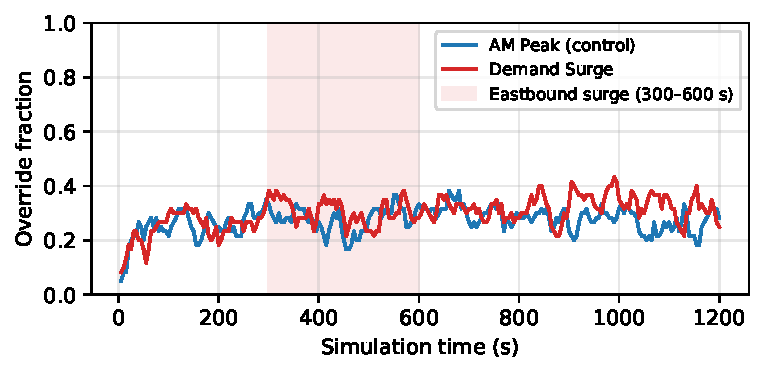
\includegraphics[width=0.8\columnwidth]{asce_gate_timeseries.pdf}
  \caption{Per-step gate-override fraction for the best curriculum checkpoint on Demand Surge versus an AM~Peak control rollout. The shaded band marks the eastbound demand surge window (300--600\,s). The override rate rises by ${\sim}5$ percentage points during the surge and persists post-surge as queues clear, while the AM~Peak control rises only gradually as the network warms up.}
  \label{fig:gate_timeseries}
\end{figure}


\section{MAPPO Hyperparameters}
\label{app:hyperparams}

\begin{table}[H]
  \centering
  \small
  \begin{tabular}{@{}ll@{}}
    \toprule
    \textbf{Parameter} & \textbf{Value} \\
    \midrule
    Hidden dimension          & 128 \\
    Hidden layers             & 2 (actor and critic) \\
    Activation                & ReLU \\
    Actor learning rate (base)       & $3 \times 10^{-4}$ \\
    Critic learning rate (base)      & $1 \times 10^{-3}$ \\
    LR scaling (parallel)    & $1/\sqrt{N_{\mathrm{workers}}}$ \\
    Optimizer                 & Adam \\
    Discount ($\gamma$)       & 0.99 \\
    GAE $\lambda$             & 0.95 \\
    PPO clip $\epsilon$       & 0.2 \\
    Entropy coefficient       & 0.01 \\
    Value loss coefficient    & 0.5 \\
    Gradient clip (max norm)  & 0.5 \\
    PPO epochs per update     & 5 \\
    Minibatch size            & 512 \\
    Gate initialization bias  & $-2.0$ (98\% follow MP) \\
    Observation normalization & Welford running mean/variance \\
    Parallel workers          & 8 (libsumo) \\
    \bottomrule
  \end{tabular}
\end{table}


\section{Person-Time-Loss Definition}
\label{app:ptl}

Person-time-loss is defined as:
\begin{equation}
  \mathrm{PTL} = \sum_{v \in \mathcal{V}} \Delta t_v^{\mathrm{loss}} \cdot w_v,
\end{equation}
where $\mathcal{V}$ is the set of all vehicles active during the episode, $\Delta t_v^{\mathrm{loss}}$ is the SUMO-reported time-loss (excess travel time over free-flow speed) for vehicle $v$, and $w_v$ is the person occupancy weight: 1.3 for cars and 30.0 for TTC buses, streetcars, and transit vehicles.


\section{Metric Definitions}
\label{app:metrics}

\begin{table}[H]
  \centering
  \small
  \begin{tabularx}{\columnwidth}{@{}l X@{}}
    \toprule
    \textbf{Metric} & \textbf{Definition} \\
    \midrule
    Person-time-loss (s) & See Appendix~\ref{app:ptl}. \\
    Vehicle delay fairness (Jain) & Jain's index~\cite{jain1984} computed over per-vehicle final time-loss values for all vehicles that complete their trip during the episode. \\
    Throughput & Number of vehicles that complete their trip within the episode. \\
    Avg trip time (s) & Mean travel time from departure to arrival over all arrived vehicles. \\
    Gate fraction & Proportion of agent-steps where the gate head selects ``override'' rather than ``follow Max-Pressure.'' \\
    \bottomrule
  \end{tabularx}
\end{table}


\section{Reward Function Iterations}
\label{app:reward_iterations}

The final \texttt{person\_objective} reward (Eq.~\ref{eq:reward_person}) was arrived at through three iterations, each addressing a specific failure mode. Table~\ref{tab:reward_ablation} summarizes the progression.

\begin{table}[H]
  \centering
  \small
  \caption{Reward function ablation on AM Peak. MAPPO/MP is the person-time-loss ratio (lower is better).}
  \label{tab:reward_ablation}
  \begin{tabular}{@{}lccl@{}}
    \toprule
    \textbf{Reward mode} & \textbf{MAPPO/MP} & \textbf{Scenario} & \textbf{Failure mode} \\
    \midrule
    \texttt{time\_loss}        & $>$1.0  & AM Peak & Too sparse; worse than Fixed-Time \\
    \texttt{objective}         & 0.93    & AM Peak & Throughput bias dominates gradient \\
    person + throughput        & $\approx$1.0  & AM Peak & Throughput amplified by normalization \\
    \texttt{person\_objective} & \textbf{0.90} & AM Peak & Selected (see Table~\ref{tab:results}) \\
    \bottomrule
  \end{tabular}
\end{table}

\paragraph{Iteration 1: \texttt{objective} (interim report).}
Combined delay, throughput, and global fairness:
$r_i = -\log(1 + d_i) + \log(1 + \tau_i) + 0.25 \cdot J(\boldsymbol{\tau})$,
where $d_i$ is waiting time at intersection $i$, $\tau_i$ is vehicle count, and $J(\boldsymbol{\tau})$ is Jain's index~\cite{jain1984} over per-agent throughputs. This enabled MAPPO to beat Fixed-Time but left it 25\% behind Max-Pressure. The throughput term $\log(1+\tau_i)$ acted as a near-constant positive bias that dominated the delay gradient, causing the policy to optimize for flow rather than delay reduction. Evaluation results were highly variable across seeds.

\paragraph{Iteration 2: Person-weighted with throughput (abandoned).}
To fix the bias, we switched to person-weighted metrics (occupancy weighting: 1.3 for cars, 30 for transit) and attempted to normalize the throughput term. Normalizing throughput into the formula amplified its relative magnitude further; the model learned to maximize flow volume while ignoring delay entirely (MAPPO/MP $\approx 1.0$).

\paragraph{Iteration 3: \texttt{person\_objective} (final).}
The key insight was that throughput should not appear in the reward at all. It was originally added because the raw \texttt{time\_loss} signal was too sparse (a lesson from the interim report). The correct fix was to make the delay signal richer by (1)~computing a per-person delay rate instead of a raw accumulator, (2)~using local NS/EW directional Jain fairness instead of global throughput fairness, and (3)~person-weighting to align with the evaluation KPI. See Section~\ref{sec:reward} for the formula.


\section{Observation and Feature Dimensions}
\label{app:obs_features}

Each agent's observation is a variable-length vector whose dimension depends on the intersection's topology:

\begin{table}[H]
  \centering
  \small
  \caption{Observation feature blocks per agent. Total dimension ranges from 9 to 43 (base) plus 6 (MP augmentation) = 15 to 49, padded to a common maximum.}
  \label{tab:obs_features}
  \begin{tabular}{@{}lll@{}}
    \toprule
    \textbf{Block} & \textbf{Size} & \textbf{Description} \\
    \midrule
    Phase one-hot    & 2--6     & Current green phase encoding \\
    Min-green flag   & 1        & 1 if phase may switch, else 0 \\
    Lane density     & 3--18    & vehicles/capacity per incoming lane, $[0,1]$ \\
    Lane queue       & 3--18    & halted vehicles/capacity per lane, $[0,1]$ \\
    MP one-hot       & 6        & Max-Pressure recommended phase (gate mode) \\
    \midrule
    \textbf{Total}   & 15--49   & Padded to max across all 12 agents \\
    \bottomrule
  \end{tabular}
\end{table}

The centralized critic receives the concatenation of all 12 agents' normalized observations (${\sim}460$ dimensions). Observation normalization uses Welford's online algorithm~\cite{welford} to maintain per-feature running mean and variance, applied separately to local (actor) and global (critic) observation streams.

The actor network (GatedActor) has $128 \times 2$ hidden units with ReLU activations. Its two output heads are:
\begin{itemize}[nosep]
  \item \textbf{Gate head}: Linear($128 \to 2$), softmax. Initialization bias $[-2.0, +2.0]$ yields ${\sim}$98\% follow-MP at start.
  \item \textbf{Phase head}: Linear($128 \to 6$), softmax with invalid-action masking (logits set to $-\infty$ for illegal phases). Valid phases range from 2 to 6 per intersection.
\end{itemize}


\section{Full Evaluation Metrics}
\label{app:full_metrics}

Table~\ref{tab:full_metrics} reports all evaluation metrics for the best curriculum checkpoint across scenarios (mean $\pm$ std, 5 seeds).

\begin{table}[H]
  \centering
  \small
  \caption{Complete evaluation metrics for \texttt{curriculum\_best} checkpoint.}
  \label{tab:full_metrics}
  \begin{tabular}{@{}llrrrr@{}}
    \toprule
    \textbf{Scenario} & \textbf{Controller} & \textbf{Avg Trip (s)} & \textbf{Arrived} & \textbf{Jain} & \textbf{Gate \%} \\
    \midrule
    \multirow{3}{*}{AM Peak}
      & Max-Pressure & $76.5 \pm 5.4$ & $631 \pm 31$ & $0.340 \pm 0.019$ & --- \\
      & Fixed-Time   & $75.1 \pm 1.9$ & $664 \pm 14$ & $0.307 \pm 0.016$ & --- \\
      & MAPPO        & $73.4 \pm 2.8$ & $688 \pm 31$ & $0.432 \pm 0.024$ & 26.7 \\
    \midrule
    \multirow{3}{*}{PM Peak}
      & Max-Pressure & $102.7 \pm 4.9$ & $542 \pm 19$ & $0.404 \pm 0.013$ & --- \\
      & Fixed-Time   & $85.6 \pm 3.3$  & $687 \pm 18$ & $0.361 \pm 0.031$ & --- \\
      & MAPPO        & $102.3 \pm 5.6$ & $604 \pm 39$ & $0.506 \pm 0.050$ & 27.4 \\
    \midrule
    \multirow{3}{*}{Demand Surge}
      & Max-Pressure & $93.4 \pm 1.8$ & $539 \pm 87$ & $0.389 \pm 0.018$ & --- \\
      & Fixed-Time   & $81.6 \pm 2.2$ & $702 \pm 14$ & $0.355 \pm 0.007$ & --- \\
      & MAPPO        & $94.7 \pm 0.6$ & $627 \pm 31$ & $0.521 \pm 0.030$ & 27.3 \\
    \midrule
    \multirow{3}{*}{Midday Mult.}
      & Max-Pressure & $93.4 \pm 3.5$ & $558 \pm 32$ & $0.369 \pm 0.040$ & --- \\
      & Fixed-Time   & $85.5 \pm 2.9$ & $605 \pm 26$ & $0.317 \pm 0.014$ & --- \\
      & MAPPO        & $92.3 \pm 6.0$ & $611 \pm 15$ & $0.477 \pm 0.021$ & 30.2 \\
    \bottomrule
  \end{tabular}
\end{table}

MAPPO achieves the lowest average trip time on AM Peak and is comparable to Max-Pressure on other scenarios. Fixed-Time achieves lower trip times on PM Peak and Demand Surge because it cycles uniformly and clears more vehicles through the network, but at the cost of substantially worse person-weighted delay and fairness. MAPPO's Jain index is 27--34\% higher than Max-Pressure across all scenarios, indicating more equitable delay distribution, though no controller approaches the proposal target of 0.8.


\section{Summary of Changes from Interim Report}
\label{app:interim_changes}

Since the interim report, several modifications have been made.

Firstly, the ASCE algorithm was upgraded to be action-gated with Max-Pressure as the base instead of a simple MAPPO algorithm. This was one of the main future works discussed in the interim report, as the intended benefit of using ASCE over Max-Pressure is that it outperforms Max-Pressure under irregular conditions, while performing at least as well as Max-Pressure under regular conditions. In the interim report, Max-Pressure used to outperform ASCE in every scenario.

Specifically, four different scenarios (AM peak, PM peak, midday multimodal---i.e.\ peak pedestrian traffic---and demand surge) were made based on real TMC corridor data for our chosen intersections, and the model was trained through curriculum training. Now, ASCE outperforms Max-Pressure under all conditions, regular or irregular. To accomplish curriculum training, batched reinforcement learning was also implemented.

This also means that the model now includes the effect of buses, pedestrians, and paralleling transit lines.


% =============================================================================
% CHECKLIST
% =============================================================================
\section*{NeurIPS Paper Checklist}

\begin{enumerate}

\item {\bf Claims}
    \item[] Question: Do the main claims made in the abstract and introduction accurately reflect the paper's contributions and scope?
    \item[] Answer: \answerYes{}
    \item[] Justification: The abstract states specific MAPPO-vs-Max-Pressure improvement percentages with paired $p$-values per scenario, which are directly supported by Table~\ref{tab:results}. The incomplete status of PIRA is stated in the abstract, in Section~\ref{sec:pira}, and in the Statement of Scope Changes.

\item {\bf Limitations}
    \item[] Question: Does the paper discuss the limitations of the work performed by the authors?
    \item[] Answer: \answerYes{}
    \item[] Justification: Section~\ref{sec:analysis} discusses PM~Peak underperformance, the tie with Actuated~Default on three of four scenarios, curriculum instability, and gate-override behaviour; Section~\ref{sec:scope} lists scope reductions relative to the proposal.

\item {\bf Theory assumptions and proofs}
    \item[] Question: For each theoretical result, does the paper provide the full set of assumptions and a complete (and correct) proof?
    \item[] Answer: \answerNA{}
    \item[] Justification: The paper reports an empirical study; no theorems or proofs are claimed.

\item {\bf Experimental result reproducibility}
    \item[] Question: Does the paper fully disclose all the information needed to reproduce the main experimental results of the paper to the extent that it affects the main claims and/or conclusions of the paper (regardless of whether the code and data are provided or not)?
    \item[] Answer: \answerYes{}
    \item[] Justification: Full hyperparameters (Appendix~\ref{app:hyperparams}), observation features (Appendix~\ref{app:obs_features}), reward iterations (Appendix~\ref{app:reward_iterations}), scenario definitions (Section~\ref{sec:scenarios}), and the exact reproduction command (\texttt{pixi run eval-matrix}) are provided along with a locked \texttt{pixi.lock} environment and the trained checkpoint.

\item {\bf Open access to data and code}
    \item[] Question: Does the paper provide open access to the data and code, with sufficient instructions to faithfully reproduce the main experimental results, as described in supplemental material?
    \item[] Answer: \answerYes{}
    \item[] Justification: All code, trained models, calibrated demand, SUMO network, and evaluation scripts are released at \url{https://github.com/yashnkapadia/ece324-TANGO}. Section~7 gives the exact \texttt{pixi install}/\texttt{pixi run eval-matrix} commands that reproduce the headline numbers from the committed best checkpoint.

\item {\bf Experimental setting/details}
    \item[] Question: Does the paper specify all the training and test details (e.g., data splits, hyperparameters, how they were chosen, type of optimizer) necessary to understand the results?
    \item[] Answer: \answerYes{}
    \item[] Justification: The training pipeline (optimizer, learning rate, rollout and update schedule, curriculum) is in Section~\ref{sec:training} and Appendix~\ref{app:hyperparams}; the evaluation protocol (5 matched seeds, paired $t$-test, baselines) is in Section~\ref{sec:results}.

\item {\bf Experiment statistical significance}
    \item[] Question: Does the paper report error bars suitably and correctly defined or other appropriate information about the statistical significance of the experiments?
    \item[] Answer: \answerYes{}
    \item[] Justification: All headline results in Table~\ref{tab:results} report mean~$\pm$~standard deviation across 5 matched random seeds, along with two-sided paired $t$-test $p$-values against Max-Pressure. The matched-seeds design is described in Section~\ref{sec:results}.

\item {\bf Experiments compute resources}
    \item[] Question: For each experiment, does the paper provide sufficient information on the computer resources (type of compute workers, memory, time of execution) needed to reproduce the experiments?
    \item[] Answer: \answerYes{}
    \item[] Justification: Section~7 reports the hardware (RTX~4070 Laptop GPU), wall-clock runtime for the full pipeline ($\sim$8~h), and the total project compute budget ($\sim$40 GPU-hours including failed runs).

\item {\bf Code of ethics}
    \item[] Question: Does the research conducted in the paper conform, in every respect, with the NeurIPS Code of Ethics \url{https://neurips.cc/public/EthicsGuidelines}?
    \item[] Answer: \answerYes{}
    \item[] Justification: The research uses only publicly available, aggregated traffic counts and open-source simulation tools. No human subjects, personal data, or dual-use models are involved.

\item {\bf Broader impacts}
    \item[] Question: Does the paper discuss both potential positive societal impacts and negative societal impacts of the work performed?
    \item[] Answer: \answerYes{}
    \item[] Justification: Section~\ref{sec:future} / the discussion in Section~\ref{sec:analysis} note both the potential benefit (reduced person-delay and improved vehicle-delay fairness) and the risk that reducing travel time can induce demand; the paper also flags that results are only validated in simulation and should not be deployed without real-world safety review.

\item {\bf Safeguards}
    \item[] Question: Does the paper describe safeguards that have been put in place for responsible release of data or models that have a high risk for misuse (e.g., pre-trained language models, image generators, or scraped datasets)?
    \item[] Answer: \answerNA{}
    \item[] Justification: The released artefacts are a traffic-signal control policy trained on aggregated public statistics and a calibrated SUMO scenario; they do not pose a misuse risk comparable to generative models or scraped datasets.

\item {\bf Licenses for existing assets}
    \item[] Question: Are the creators or original owners of assets (e.g., code, data, models), used in the paper, properly credited and are the license and terms of use explicitly mentioned and properly respected?
    \item[] Answer: \answerYes{}
    \item[] Justification: SUMO (EPL-2.0), SUMO-RL (MIT), the MAPPO reference implementation, and the City of Toronto TMC dataset are cited in the text and bibliography; the vendored fork of SUMO-RL preserves the upstream MIT license in-tree.

\item {\bf New assets}
    \item[] Question: Are new assets introduced in the paper well documented and is the documentation provided alongside the assets?
    \item[] Answer: \answerYes{}
    \item[] Justification: The trained ASCE checkpoint, calibrated demand scenarios, vendored sumo-rl modifications, and the Demand Studio UI are released in the repository with top-level \texttt{README.md}, \texttt{ASCE.md}, \texttt{DATA.md}, and \texttt{PIRA.md} documenting layout, reproduction commands, and limitations.

\item {\bf Crowdsourcing and research with human subjects}
    \item[] Question: For crowdsourcing experiments and research with human subjects, does the paper include the full text of instructions given to participants and screenshots, if applicable, as well as details about compensation (if any)?
    \item[] Answer: \answerNA{}
    \item[] Justification: The project does not involve crowdsourcing or human subjects.

\item {\bf Institutional review board (IRB) approvals or equivalent for research with human subjects}
    \item[] Question: Does the paper describe potential risks incurred by study participants, whether such risks were disclosed to the subjects, and whether Institutional Review Board (IRB) approvals (or an equivalent approval/review based on the requirements of your country or institution) were obtained?
    \item[] Answer: \answerNA{}
    \item[] Justification: The project does not involve human subjects, so no IRB review was required.

\item {\bf Declaration of LLM usage}
    \item[] Question: Does the paper describe the usage of LLMs if it is an important, original, or non-standard component of the core methods in this research? Note that if the LLM is used only for writing, editing, or formatting purposes and does \emph{not} impact the core methodology, scientific rigor, or originality of the research, declaration is not required.
    \item[] Answer: \answerYes{}
    \item[] Justification: LLMs were used only as a development assistant (code scaffolding, debugging, and prose editing), not as part of the core method. See the Generative AI Usage Statement below for details.

\end{enumerate}


% =============================================================================
% GENERATIVE AI STATEMENT
% =============================================================================
\section*{Generative AI Usage Statement}

Claude Code (Anthropic, Claude Opus) was used as a development assistant throughout this project for code implementation and debugging of the ASCE training pipeline, reward function iteration, and parallel training infrastructure. All generated code was reviewed, tested, and modified by the authors. Claude Code was not used to generate experimental results or evaluation metrics---all reported numbers come from SUMO simulation runs.


\end{document}
